%
% 3-differentialoperatoren.tex -- Differentialoperatoren
%
% (c) 2024 Prof Dr Andreas Müller
%
\section{Differentialoperatoren
\label{buch:koordinaten:section:differentialoperatoren}}
\kopfrechts{Differentialoperatoren}
Der Tangentialvektor ist in
Definition~\ref{buch:koordinaten:tangentialvektoren:def:tangentialvektor}
sehr abstrakt definiert worden.
Tangentialvektoren sind das, was tangentialen Kurven gemeinsam ist,
also der Berührpunkt, die ``Richtung'' und ``Geschwindigkeit''.
Es ist aber nur indirekt mit Hilfe eines Koordinatensystems möglich, sich 
einen Tangentialvektor als einen ``Pfeil'' vorzustellen.
Richtung und Geschwindigkeit kann man aber auch dadurch detektieren, dass
man bestimmt, wie schnell sich eine Messgrösse, die von den Koordinaten
abhängig, ändert.
Die instantane Änderung einer Funktion ein einem Punkt ist so etwas
wie eine Ableitung.
In diesem Abschnitt soll daher gezeigt werden, dass man sich
Tagentialvektoren auch als Differentialoperatoren vorstellen
kann, die Funktionen ableiten können.

%
% Ableitung entlang einer Kurve
%
\subsection{Ableitung entlang einer Kurve}
Sei $X$ eine Menge versehen mit einem Koordinatensystem
$\varphi\colon X\to \mathbb{R}^n$ und sei ausserdem 
$f\colon X\to\mathbb{R}$ eine reellwertige Funktion definiert
auf $Y$.
Mithilfe des Koordinatensystems ist es möglich, die Funktion $f$
durch die Koordinaten $x^1,\dots,x^n$ als
\[
f(x^1,\dots,x^n) = f\circ\varphi^{-1} (x^1,\dots,x^n)
\]
auszudrücken.

Bereits in
Abschnitt~\ref{buch:koordinaten:koordinaten:subsection:koordinatenwechsel}
wurde erklärt, was es heisst, dass die Funktion $f$ stetig differenzierbar
ist.
Die Ableitungen der Funktion $f\circ\varphi^{-1}$ nach allen Koordinaten
$x^k$ müssen stetig sein.
Wir nehmen im folgenden an, dass die Funktion $f$ stetig differenzierbar
ist.

Sei jetzt eine differenzierbare Kurve in $X$ gegeben, die wir
der Einfachheit halber als eine differenzierbare Abbildung
\[
\gamma\colon (-\varepsilon,\varepsilon) \to X
\]
schreiben wollen und damit den Komplikationen durch verschiedene
Koordinatensysteme auf dem eindimensionalen Definitionsbereich der
Kurve für die folgende Untersuchung ignorieren.
Differenzierbarkeit bedeutet, dass die Zusammensetzung von $\gamma$
mit der Koordinatenabbildung $\varphi$ stetig differenzierbar ist.
Wir schreiben auch $x^i(t) = \varphi^i\circ\gamma(t)$ für die Koordinaten
eines Punktes, der sich auf der Kurve bewegt.

Die Zusammensetzung der Funktion $f$ mit der Kurve $\gamma$ ist eine
differenzierbare Funktion
\[
f\circ\gamma
\colon
(-\varepsilon,\varepsilon) \to \mathbb{R}
:
t
\mapsto
f(x^1(t),\dots,x^n(t)).
\]
Die Ableitung
\[
\frac{d}{dt} f(\gamma(t))
\bigg|_{t=0}
=
\frac{d}{dt} f(x^1(t),\dots,x^n(t))
\bigg|_{t=0}
\]
an der Stelle $t=0$ heisst die Ableitung von $f$ entlang der Kurve
an der Stelle $\gamma(0)$.
Sie kann mit der Kettenregel als
\begin{equation}
\frac{d}{dt} f(\gamma(t))
\bigg|_{t=0}
=
\frac{\partial f}{\partial x_k}(x^1(0),\dots,x^n(0))
\cdot
\frac{dx^k}{dt}(0)
\label{buch:koordinaten:differentialoperatoren:eqn:kurvenableitung}
\end{equation}
berechnet werden (man beachte die einsteinsche Summenkonvention).
Aus der linken Seite der Formel ist auch bereits klar, dass diese
Ableitung unabhängig ist vom gewählten Koordinatensystem auf $X$.

%
% Tangentialvektoren als Differentialoperatoren
%
\subsection{Tangentialvektoren als Differentialoperatoren}
Man erwartet, dass die Ableitung entlang der Kurve an der Stelle
$\gamma(0)$ eine lokale Eigenschaft ist, dass also nur der Verlauf
der Kurve in einer beliebig kleinen Umgebung des Punktes $\gamma(0)$
eine Rolle spielt.
Eine andere Kurve $\tilde{\gamma}\colon(-\varepsilon,\varepsilon)\to X$,
die in $0$ tangential ist an die Kurve $\gamma$, sollte zur gleichen
Ableitung führen.
Wir schreiben sie auch $\tilde{\gamma}^i(t) = \tilde{x}^i(t)$.
Tatsächlich besagt die rechte Seite von
\eqref{buch:koordinaten:differentialoperatoren:eqn:kurvenableitung},
dass die Ableitung nur von den Ableitungen
\[
\dot{x}^i(0)
=
\frac{d\gamma^i}{dt}(0)
=
\frac{d\tilde{\gamma}^i}{dt}(0)
=
\dot{\tilde{x}}^i(0)
\]
abhängt.
Dies sind aber die Komponenten des Tangentialvektors.
Die Ableitung einer Funktion entlang einer Kurve verwendet von
der Kurve nur den Tangentialvektor.

\begin{definition}[Tangentialvektor als Differentialoperator]
Sei $f\colon X\to\mathbb{R}$ eine differenzierbare Funktion und
$V$ ein Tangentialvektor im Punkt $x_0\in X$.
Dann ist
\[
V\cdot f(x_0)
=
\frac{d}{dt} f(\gamma(t))\bigg|_{t=0}
\]
für jede Kurve $\gamma(t)$ mit dem Tangentialvektor $V=\dot{\gamma}(0)$
an der Stelle $t=0$.
\end{definition}

Tangentialvektoren können also als Differentialoperatoren betrachtet
werden.

%
% Partielle Ableitungensoperatoren
%
\subsection{Partielle Ableitungsoperatoren}
Die Koordinatenlinien von
Abschnitt~\ref{buch:koordinaten:tangentialvektoren:subsection:koordinatenlinien}
sind Kurven in $X$.
Die Kurve
\[
\varphi\circ\gamma
\colon
(-\varepsilon,\varepsilon)
\to
\mathbb{R}^n
:
t\mapsto (x_0^1,\dots,x_0^k+t,\dots,x_0^n)
\]
durch den Punkt $x_0$ mit den Koordinaten $(x_0^1,\dots,x_0^n)$
hat als Tangentialvektor den $k$-ten Standardbasisvektor.
Die Ableitung einer Funktion $f$ entlang dieser Kurve ist
\begin{align*}
\frac{d}{dt}
f(x_0^1,\dots,x_0^k+t,\dots,x_0^n)
\bigg|_{t=0}
&=
\frac{\partial f}{\partial y^k}(x_0^1,\dots,x_0^n).
\end{align*}
Man kann daher den $k$-ten Standardbasisvektor im Tangentialraum
des Punktes $y_0$ mit dem Operator der partiellen Ableitung nach
der Koordinate $y^k$ identifizieren.

\begin{satz}
In einem Koordinatensystem $(X,\varphi)$ auf $X$ bilden 
die partiellen Ableitungsoperatoren 
\[
e_k
\mapsto
\partial_k = \frac{\partial}{\partial x^k}
\]
nach den Koordinaten eine Basis.
\end{satz}

Dem Tangentialvektor mit den Komponenten $u^i$ im gegebenen
Koordinatensystem entspricht also der Differentialoperator
\[
u^k\partial_i = u^k\frac{\partial}{\partial x^k},
\]
also eine Linearkombination der partiellen Ableitungsoperatoren
(einsteinsche Summenkonvention).
Der Index $k$ im Nenner des Ableitungsoperators gilt als unterer
Index, denn die zugehörigen Koeffizienten transformieren sich
wie Vektorkomponenten.

%
% Ableitung eines Vektors?
%
\subsection{Ableitung eines Vektors?
\label{buch:koordinaten:diffop:subsection:vektorableitung}}
Kann man einen Tangentialvektor ableiten?
Ein Tangentialvektor an eine $n$-dimensionale Mannigfaltigkeit wurde
definiert als eine Klasse von Kurven, die die gleiche Ableitung in
einem Punkt haben.
In einem Koordinatensystem konnte ein Tangentialvektor mit einem
Vektor in $\mathbb{R}^n$ identifiziert werden.
Später wurde dann erkannt, dass ein solcher Tangentialvektor als
Ableitungsoperator betrachtet werden kann, der auf Funktionen
wirkt.
In einem Koordinatensystem kann ein Tangentialvektor $X$ als
ein Ableitungsoperator
\[
X
=
\sum_{i=1}^n
X^i \frac{\partial}{\partial x^i}
\]
geschrieben werden.

Betrachtet man nicht nur einen Tangentialvektor in einem einzelnen
Punkt, sondern ein Vektorfeld, welches jedem Punkt der Mannigfaltigkeit
einen Vektor zuordnet, dann lässt sich diese Vektorfeld in Koordinaten
als ortsabhängiger Vektor
\[
X(x)
=
\sum_{i=1}^n
X^i(x)
\frac{\partial}{\partial x^i}
\]
schreiben.
Auf eine Funktion $f$ angewendet ergibt sich die Funktion
\[
(X\cdot f)(x)
=
\sum_{i=1}^n X^i(x)\frac{\partial f}{\partial x^i}(x).
\]
Die Komponenten $X^i$ erfüllen die korrekten Transformationseigenschaften
für einen Vektor.

Für einen Vektor $Y$ mit der Komponentendarstellung
\[
Y
=
\sum_{i=1}^n
Y^i\frac{\partial}{\partial x^i}
\]
an einer Stelle $x$ stellt sich jetzt die Frage, ob man $Y$ als
Differentialoperator auf das Vektorfeld $X$ anwenden und daraus
wieder einen Tangentialvektor bekommen kann.
Das Resultat müsste wieder ein Differentialoperator erster Ordnung
sein.
Die Zusammensetzung der beiden Differentialoperatoren $Y$ und $X(x)$
angewendet auf eine Funktion $f$ ist
\begin{align}
Y\cdot(X\cdot f)
&=
\sum_{i=1}^n Y^i\frac{\partial}{\partial x^i}
\sum_{k=1}^n
X^k(x)
\frac{\partial f}{\partial x^k}f(x)
\notag
\\
&=
\sum_{i,k=1}^n
Y^i
\frac{\partial X^k}{\partial x^i}(x)
\frac{\partial f}{\partial x^k}(x)
+
\sum_{i,k=1}^n
Y^i
X^k(x)
\frac{\partial^2 f}{\partial x^i\,\partial x^k}(x).
\label{buch:koordinaten:diffop:eqn:vektorableitung}
\end{align}
Der erste Term könnte als ein Vektor mit den Komponenten 
\[
\sum_{i=1}^n
Y^i\frac{\partial X^k}{\partial x^i}(x)
\]
betrachtet werden, der zweite Term ist aber definitiv kein
Differentialoperator erster Ordnung.
Man kann also nicht erwarten, dass sich Vektoren ableiten lassen.

Der tiefere Grund dafür ist, dass eine Ableitung von Vektoren verlangt,
dass man Vektoren an verschiedenen Stellen miteinander verrechnen kann.
Diese Voraussetzung ist aber nicht selbstverständlich.
%
% fig-parallel.tex
%
% (c) 2025 Prof Dr Andreas Müller
%
\begin{figure}
\centering
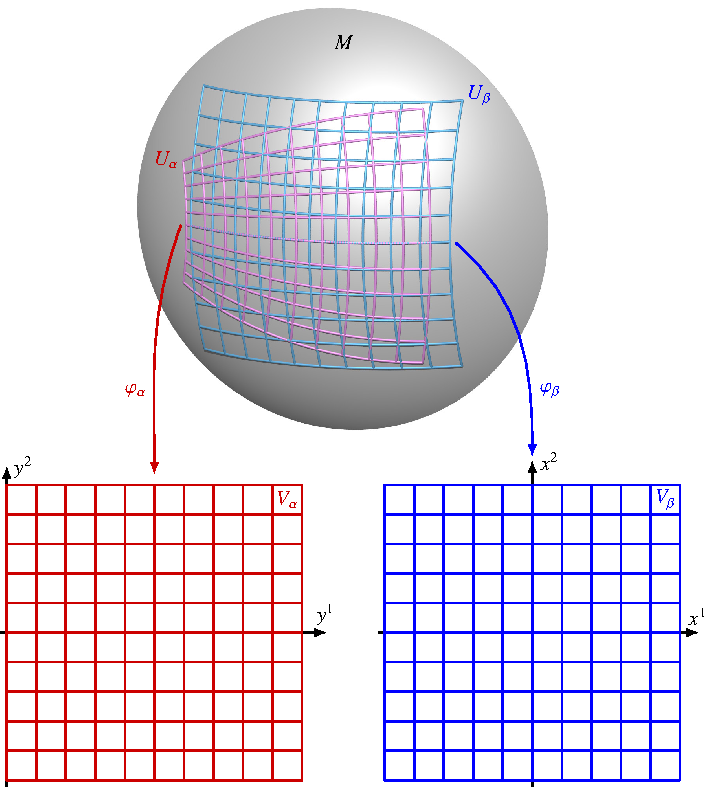
\includegraphics{chapters/020-koordinaten/images/parallel.pdf}
\caption{Je nach Koordinatensystem (Karte) hat ein entlang einer
Koordinatenlinie in der Karte parallel transportierter Vektor
eine ganz andere Richtung.
Dies illustriert, dass es ohne das zusätzliche Konzept eines
Zusammenhangs nicht möglich ist, benachbarte Vektoren zu vergleichen
oder Vektoren abzuleiten.
\label{buch:koordinaten:diffop:fig:transport}}
\end{figure}
%
In einem bestimmten Koordinatensystem kann man zwar einen Vektor
von einem Punkt zu einem anderen Punkt verschieben.
In Abbildung~\ref{buch:koordinaten:diffop:fig:transport}
ist dargestellt, wie ein Vektor, der in kartesischen Koordinaten
parallel verschoben ist, in Polarkoordinaten nach einer undurchschaubaren
Vorschrift transformiert wird.
Der Transport von Vektoren entlang einer Kurve ist also keine
Selbstverständlichkeit, er erfordert ein zusätzliches mathematisches
Hilfsmittel.
Ein Zusammenhang, wie er in Kapitel~\ref{chapter:zusammenhang} definiert
wird, schafft diese Möglichkeit.

%
% Die Lie-Ableitung
%
\subsection{Lie-Ableitung}
Abschnitt~\ref{buch:koordinaten:diffop:subsection:vektorableitung}
hat gezeigt, dass die Zusammensetzung zweier Vektorfelder, betrachtet
als Differentialoperatoren, kein Differentialoperator erster Ordnung
sein kann.
Aus technischer Sicht war der Grund der zweite Term 
in~\eqref{buch:koordinaten:diffop:eqn:vektorableitung}
mit den zweiten Ableitungen.
Für zwei Vektorfelder $X$ und $Y$ mit Komponenten $X^i(x)$ und
$Y^k(x)$ ergibt sich bei Anwendung der
Formel~\eqref{buch:koordinaten:diffop:eqn:vektorableitung}
der gleiche Term mit zweiten Ableitungen.
Die Differenz enthält diesen Term daher nicht mehr:
\begin{align*}
Y\cdot(X\cdot f)
-
X\cdot(Y\cdot f)
&=
\sum_{i,k=1}^n
Y^i(x)\frac{\partial X^k}{\partial x^i}(x) \frac{\partial f}{\partial x^k}(x)
-
\sum_{i,k=1}^n
X^i(x)\frac{\partial Y^k}{\partial x^i}(x) \frac{\partial f}{\partial x^k}(x)
\\
&=
\sum_{k=1}^n
\sum_{i=1}^n
\biggl(
Y^i(x)\frac{\partial X^k}{\partial x^i}(x)
-
X^i(x)\frac{\partial Y^k}{\partial x^i}(x)
\biggr)
\frac{\partial f}{\partial x^k}(x).
\end{align*}
Da darin nur noch erste Ableitungen vorkommen, ist dies wieder
ein Differentialoperator erster Ordnung, der als Vektor
geschrieben werden kann.

\begin{definition}[Lie-Ableitung]
\label{buch:koordinaten:diffop:def:lieableitung}
Der Differentialoperator 
\[
f\mapsto
X\cdot(Y\cdot f)
-
Y\cdot(X\cdot f)
\]
ist ein Differentialoperator erster Ordnung.
Er heisst die {\em Lie-Klammer} und wird auch $[X,Y]$
geschrieben.
\end{definition}

\begin{satz}[Lie-Algebra]
\label{buch:koordinaten:diffop:satz}
Die Lie-Klammer der Vektorfelder $X$, $Y$ und $Z$ erfüllt
\begin{enumerate}
\item $[X,X]=0$
\item $[X, [Y, Z]] + [Y, [Z, X]] + [Z, [X, Y]] = 0$
\end{enumerate}
\end{satz}

Die zweite Formel ist unter dem Namen {\em Jacobi-Identität} bekannt.
Die Rechenregeln von Satz~\ref{buch:koordinaten:diffop:satz} besagen,
dass die Vektorfelder eine sogenannten {\em Lie-Algebra} bilden.

\begin{proof}
Beide Formeln können sofort mit Hilfe der
Definition~\ref{buch:koordinaten:diffop:def:lieableitung}
berechnet werden.
\begin{enumerate}
\item
\(
[X,X]\cdot f = X\cdot X\cdot f - X\cdot X\cdot f
=
0
\).
\item
Ein Term der Jacobi-Identität ist nach
\definecolor{cyan}{rgb}{0,0.8,0.8}
\begin{align*}
[X,[Y,Z]]\cdot f
&=
X\cdot [Y, Z]\cdot f
-
[Y, Z]\cdot X\cdot f
\\
&=
X\cdot Y\cdot Z\cdot f
-
X\cdot Z\cdot Y\cdot f
-
Y\cdot Z\cdot X\cdot f
+
Z\cdot Y\cdot X\cdot f.
\intertext{Dazu werden jetzt die Terme mit zyklisch vertauschten
$X$, $Y$ und $Z$ hinzuaddiert, dann ergibt sich die linke Seite
der Jacobi-Identität:}
\text{LHS}
&=
{\color{darkred}X\cdot Y\cdot Z}\cdot f
-
{\color{blue}X\cdot Z\cdot Y}\cdot f
-
{\color{darkgreen}Y\cdot Z\cdot X}\cdot f
+
{\color{orange}Z\cdot Y\cdot X}\cdot f
\\
&+
{\color{darkgreen}Y\cdot Z\cdot X}\cdot f
-
{\color{violet}Y\cdot X\cdot Z}\cdot f
-
{\color{cyan}Z\cdot X\cdot Y}\cdot f
+
{\color{blue}X\cdot Z\cdot Y}\cdot f
\\
&+
{\color{cyan}Z\cdot X\cdot Y}\cdot f
-
{\color{orange}Z\cdot Y\cdot X}\cdot f
-
{\color{darkred}X\cdot Y\cdot Z}\cdot f
+
{\color{violet}Y\cdot X\cdot Z}\cdot f.
\end{align*}
Die Terme gleicher Farbe heben sich weg, was die Jacobi-Identität
beweist.
\qedhere
\end{enumerate}
\end{proof}

Ein Ableitungsoperator ist ein linearer Operator, der auch eine
Produktregel erfüllt.
Zum Beispiel gilt für ein Produkt von Funktionen $f\cdot g$
\begin{align*}
X\cdot (f\cdot g)
&=
\sum_{k=1}^n
X^k
\frac{\partial (f\cdot g)}{\partial x^k}(x)
\\
&=
\sum_{k=1}^n
X^k
\biggl(
\frac{\partial f}{\partial x^k}(x)\cdot g(x)
+
f(x)
\cdot
\frac{\partial g}{\partial x^k}(x)
\biggr)
\\
&=
\biggl(
\sum_{k=1}^n
X^k
\frac{\partial f}{\partial x^k}(x)
\biggr)\cdot g(x)
+
f(x)
\cdot
\biggl(
\sum_{k=1}^n
X^k
\frac{\partial g}{\partial x^k}(x)
\biggr)
\\
&=
(X\cdot f)\cdot g
+
f\cdot(X\cdot g).
\end{align*}
Diese Eigenschaft heisst

\begin{definition}[Derivation]
\label{buch:koordinaten:diffop:def:derivation}
Sei $A$ eine reelle Algebra.
Eine Derivation auf $A$ ist eine lineare Abbildung $d\colon A\to A$,
die
\[
d(f\cdot g)
=
(df)\cdot g
+
f\cdot dg
\]
erfüllt.
\end{definition}

Die Lie-Klammer hat die Eigenschaft einer Derivation auch dann,
wenn man sie auf ein Produkt $fY$ einer Funktion und eines Vektorfeldes
anwendet.
Dazu berechnen wir:
\begin{align}
[X,fY]\cdot g
&=
X\cdot((fY)\cdot g)
-
(fY)\cdot(X\cdot g)
\notag
\\
&=
X\cdot(f (Y\cdot g))
-
fY\cdot (X\cdot g)
\notag
\\
&=
(X\cdot f)(Y\cdot g))
+
f(X\cdot (Y\cdot g))
-
fY\cdot (X\cdot g)
\notag
\\
&=
(X\cdot f)(Y\cdot g)
+
f([X,Y]\cdot g).
\notag
\intertext{Geschrieben als Operatoren (ohne die Funktion $g$) ist dies}
[X,fY]
&=
(X\cdot f)Y + f[X,Y].
\label{buch:koordinaten:diffop:eqn:lieprodukt}
\end{align}
In den beiden Termen der letzten Gleichungen wirkt die zu $X$
gehörige Ableitung jeweils auf einem der Faktoren wie in der Produktregel.
Die Analogie kann noch etwas offensichtlicher gemacht werden, wenn
wir die folgende Notation wählen.

\begin{definition}
\label{buch:koordinaten:diffop:def:lieableitung}
Sei $X$ ein Vektorfeld, dann ist die zum Vektorfeld $X$ gehörige
{\em Lie-Ableitung} $L_X$ auf einer Funktion $f$ definiert durch
\index{Lie-Ableitung}%
$L_Xf=X\cdot f$, und auf einem Vektorfeld $Y$ durch $L_XY=[X,Y]$.
\end{definition}

Mit dieser Schreibweise wird die Gleichung
\eqref{buch:koordinaten:diffop:eqn:lieprodukt}
zu
\[
L_X(fY)
=
(L_Xf)\cdot Y
+
f\cdot L_XY,
\]
die genau die Form einer Produktregel hat.

Mit der Schreibweise von Definition
\ref{buch:koordinaten:diffop:def:lieableitung} kann die
Jacobi-Identität in eine übersichtlichere Form
gebracht werden.
Dazu schreibt man sie zunächst so um, dass $Z$ jeweils ganz rechts steht:
\[
[X,[Y,Z]] - [Y,[X,Z]] - [[X,Y],Z] = 0.
\]
Darin schreiben wir alle Lie-Klammern als Lie-Ableitungen, ausser der Klammer
$[X,Y]$, und erhalten
\begin{equation}
L_X\circ L_Y - L_Y\circ L_X
=
L_{[X,Y]}.
\label{buch:koordinaten:diffop:eqn:liekommutator}
\end{equation}
Die linke Seite von
\eqref{buch:koordinaten:diffop:eqn:liekommutator}
wird auch als Kommutator 
\[
[L_X,L_Y]
:=
L_X\circ L_Y - L_Y\circ L_X
\]
bezeichnet.
Nach \eqref{buch:koordinaten:diffop:eqn:liekommutator}
ist also der Kommutator der Operatoren $L_X$ und $L_Y$
die Lie-Ableitung mit dem Vektorfeld $[X,Y]$.



